\documentclass{summarysheet}

\begin{document}

\maketitle{12}{Gravity}


\begin{multicols}{2}

\begin{topicbox}{Newton's Law of Gravity}

\noindent Every object in the universe attracts every other object with a \emph{gravitational force}
\begin{eqbox}
F_\text{1 on 2} = F_\text{2 on 1} = \frac{G m_1 m_2 }{r^2},
\end{eqbox}
\noindent where 
\[
G = 6.67\times 10^{-11} \text{ N\,m$^2$/kg$^2$}
\]
is called the \emph{gravitational constant}.
\begin{center}
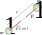
\includegraphics[scale=0.6]{fig_grav.pdf}
\end{center}

\end{topicbox}

\begin{topicbox}{Surface Gravity}

\noindent The free fall acceleration of an object at the surface of a planet of mass $M$ is 
\[
g = \frac{GM}{r^2},
\]
where $r$ is measured from the centre of the planet.

\end{topicbox}

\begin{topicbox}{Gravitational Potential Energy}

\noindent The gravitational potential energy of a system of two objects is given by
\begin{eqbox}
U_G = -\frac{Gm_1 m_2}{r}.
\end{eqbox}
\noindent Notes:
\begin{itemize}
\item This looks a bit like the force law, but it has a minus sign (see below) and only $r$ on the bottom.
\item The zero point is defined in this case to be when the two objects are separated by infinity (so $U_G = 0$ when $r = \infty$).
\item Only when the height above the surface of a planet is much less than the radius of the planet, $y \ll R$, does this reduce to the more familiar
\[
U_G = mgy.
\]
\end{itemize}

\end{topicbox}

\begin{topicbox}{Circular Orbits}

\noindent If a satellite of mass $m$ orbits a planet of mass $M$ in a circular orbit of radius $r$, Newton's second law says the speed of the satellite is
\begin{eqbox}
v = \sqrt{\frac{GM}{r}}.
\end{eqbox}

\begin{center}
\includegraphics[scale=0.6]{fig_circ.pdf}
\end{center}

\end{topicbox}

\begin{topicbox}{Kepler's Third Law}

\noindent The \emph{period} of an orbit is related to its radius by
\begin{eqbox}
T^2 = \left( \frac{4\pi^2}{GM} \right) r^3.
\end{eqbox}
\noindent This is called \emph{Kepler's third law.}

\end{topicbox}





\end{multicols}





\makebanner{Mechanics}

\end{document}




